Die Ortsänderung in jedem Stück ist die Fläche zwischen dem $v(t)$-Graphen und der $t$-Achse, über der Achse positiv, unter der Achse negativ:
\begin{center}
\begin{tabular}{c|c|c|c}
Stück & $v$ & Fläche $\Delta s$ & $s$ am Ende \\
\hline
1 (0--\SI{2}{\second}) & $+3$ & \SI{6}{\meter} & \SI{6}{\meter} \\
2 (2--\SI{3}{\second}) & $3 \to 0$ & \SI{1.5}{\meter} & \SI{7.5}{\meter} \\
3 (3--\SI{4}{\second}) & $0 \to -3$ & \SI{-1.5}{\meter} & \SI{6}{\meter} \\
4 (4--\SI{6}{\second}) & $-3$ & \SI{-6}{\meter} & \SI{0}{\meter}
\end{tabular}
\end{center}
\begin{abcliste}
\abc $\result{\text{Stück 4}}$ (von \tThreeO\ bis \tEO) ist falsch. Die Stücke 1 bis 3 stimmen: eine Gerade, dann eine Parabel bis zum Maximum bei \SI{3}{\second} (dort ist $v = 0$) und eine Parabel, die immer steiler abfällt.

\abc Im Stück 4 ist $v = \SI{-3}{\meter\per\second}$: Der Körper fährt rückwärts, $s$ muss abnehmen. Der Schüler hat die Fläche unter der Achse $\result{\text{positiv gezählt}}$ und den Graphen mit der Steigung $+3$ statt $-3$ weitergezeichnet. Er hätte merken können, dass sein Graph bei \tThreeO\ einen Knick hat, obwohl $v(t)$ dort nicht springt. Richtig ist
\begin{align}
 \Delta s_4 &= \dFourF = \dFour \\
 s(t_\mathrm{e}) &= \sEndF = \sEnd \approx \result{\SI{0}{\meter}}
\end{align}
Der Körper ist bei \tEO\ wieder am Startort (blau: richtig, rot gestrichelt: Skizze des Schülers):
\begin{center}
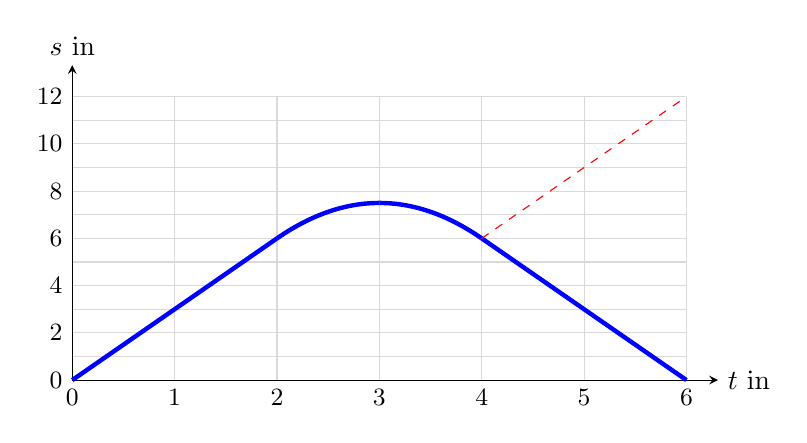
\begin{tikzpicture}[>=stealth, x=1.3cm, y=0.3cm]
 \draw[gray!30] (0,0) grid[xstep=1, ystep=1] (6,12);
 \draw[->] (0,0) -- (6.308,0) node[right] {$t$ in \si{\second}};
 \draw[->] (0,0) -- (0,13.333) node[above] {$s$ in \si{\meter}};
 \foreach \tk in {0,1,2,3,4,5,6} \node[below] at (\tk,0) {\small $\tk$};
 \foreach \yk in {0,2,4,6,8,10,12} \node[left] at (0,\yk) {\small $\yk$};
 \draw[ultra thick, blue] (0,0) -- (2,6);
 \draw[ultra thick, blue, domain=2:3, samples=30] plot (\x, {6+3*(\x-2)-1.5*(\x-2)*(\x-2)});
 \draw[ultra thick, blue, domain=3:4, samples=30] plot (\x, {7.5-1.5*(\x-3)*(\x-3)});
 \draw[ultra thick, blue] (4,6) -- (6,0);
 \draw[red, dashed] (4,6) -- (6,12);
\end{tikzpicture}
\end{center}
\end{abcliste}
